\documentclass[10pt]{article}
\usepackage[margin=1in]{geometry}
\usepackage{graphicx}
\usepackage{booktabs}
\usepackage{natbib}
\usepackage{xcolor}
\usepackage{placeins}
\graphicspath{{figs/}}
\newcommand{\verify}[1]{\textcolor{red}{[VERIFY: #1]}}
\title{Conditional VAEs for Direction-Conditioned Neural Population Activity}
\author{\verify{Add author name}}
\date{\verify{Add submission date}}

\begin{document}
\maketitle

\section{Motivation}
\begin{itemize}
  \item \verify{Write the motivation and research question in your own words.}
  \item The model is a conditional variational autoencoder (cVAE) \citep{kingma2014autoencoding}.
\end{itemize}

\section{Data}
\begin{itemize}
  \item The toy problem represents two simulated neuron rates, conditional on one of eight reach directions.
  \item The real experiment uses MC\_RTT: M1 spike trains and reaching kinematics from a macaque performing a self-paced random-target task \citep{odoherty2020dataset,makin2018superior,pei2021nlb}.
  \item \verify{Confirm all dataset wording, version information, and the final citation details against the primary source.}
\end{itemize}

\section{Method}
\begin{itemize}
  \item \verify{Describe preprocessing, the cVAE architecture, objective, training procedure, and latent-size sweeps.}
  \item \verify{Report exact hyperparameters from the final run.}
\end{itemize}

\section{Toy conditional manifold}
\begin{itemize}
  \item \verify{Interpret the real-versus-generated geometry and the effect of latent size.}
\end{itemize}
\begin{figure}[ht]
  \centering
  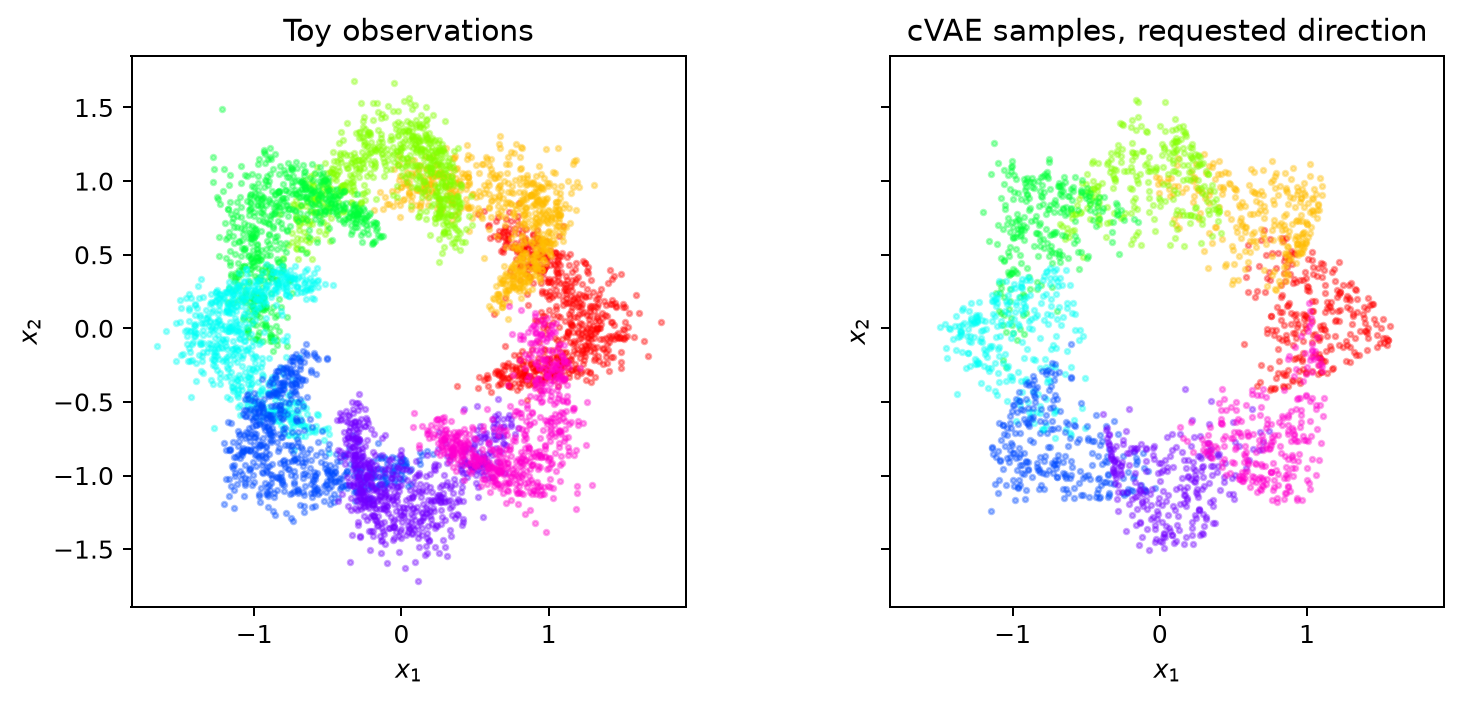
\includegraphics[width=.9\linewidth]{toy_data_and_samples.png}
  \caption{\verify{Describe the toy observations and conditional samples.}}
\end{figure}
\begin{figure}[ht]
  \centering
  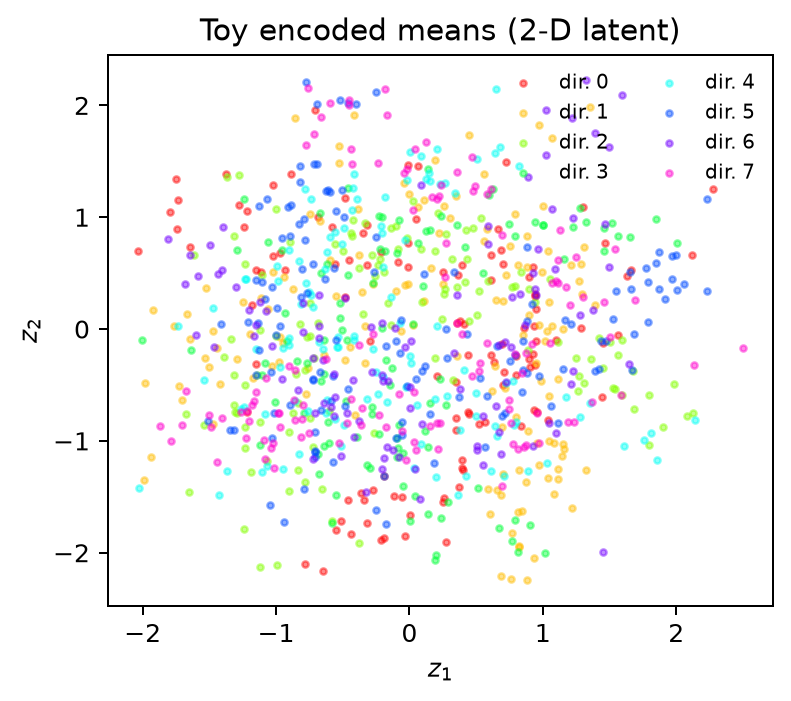
\includegraphics[width=.46\linewidth]{toy_latent.png}
  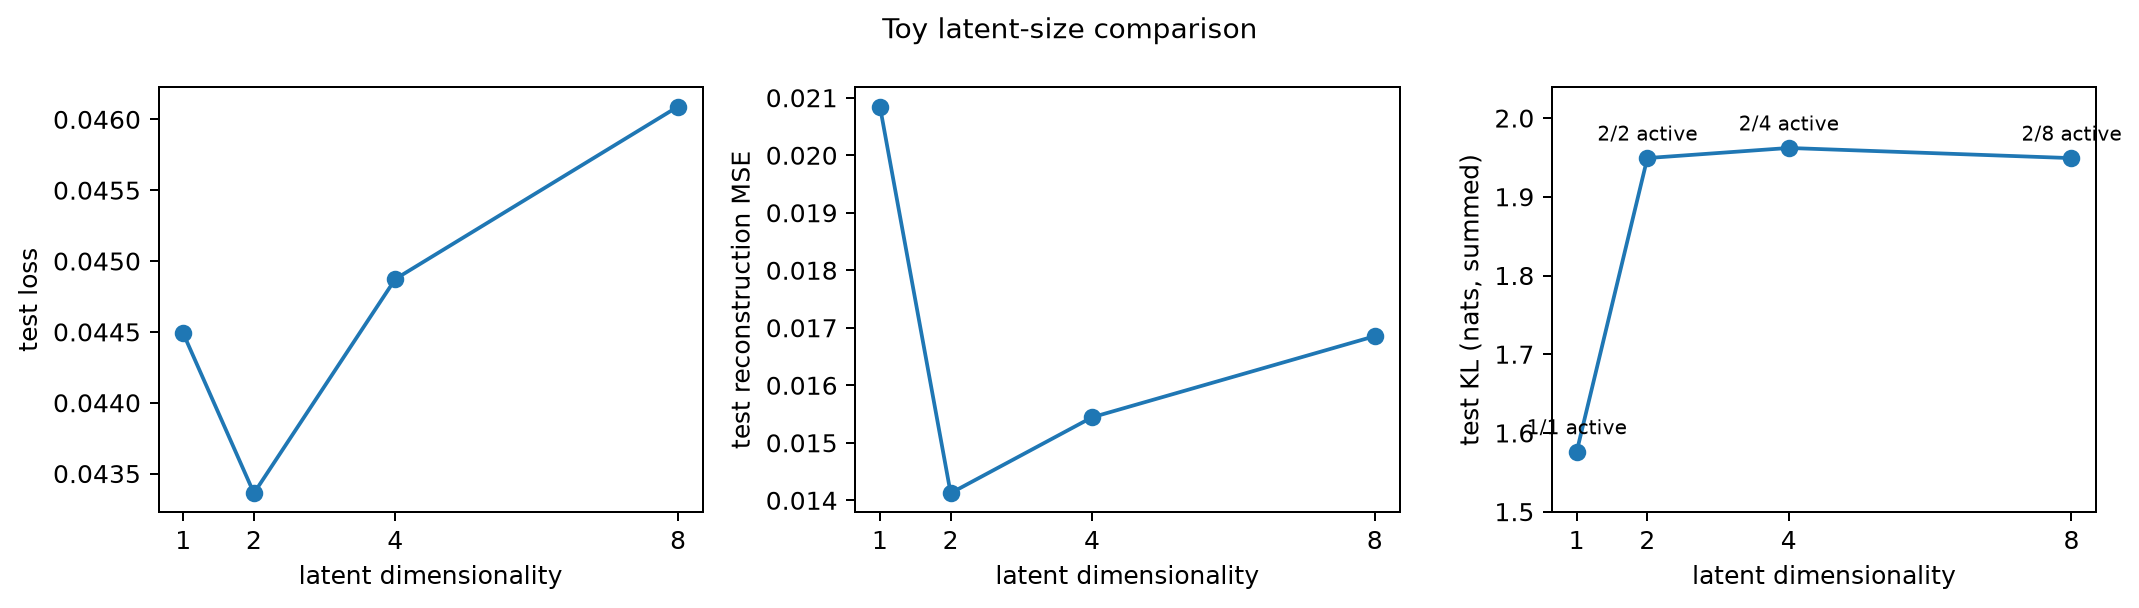
\includegraphics[width=.46\linewidth]{toy_latent_sweep.png}
  \caption{\verify{Describe the toy latent representation and latent-size comparison.}}
\end{figure}

\FloatBarrier\section{MC\_RTT population activity}

This section analyzes the MC\_RTT recording used here \citep{odoherty2020dataset,makin2018superior,pei2021nlb}.
In this experiment, each example is a 200-ms window centered on peak finger speed within a source-provided 600-ms chunk.
The input comprises log1p Gaussian-smoothed firing rates from 48 held-in primary motor cortex (M1) units in ten 20-ms bins.
The cVAE is conditioned on one of eight peak-velocity directions.
We use the source-provided split of 810 training and 270 validation chunks, so the reported validation results are evaluated on held-out chunks.
This preserves the dataset's chunk-level partition rather than creating a new random split from the same recording.

\subsection{Validation performance and latent capacity}

Increasing the latent space from 2 to 8 to 16 dimensions improves the final held-out standardized-feature reconstruction MSE from 0.877 to 0.824 to 0.766, respectively.
The corresponding total validation losses were 0.885, 0.850, and 0.811 (Figure~\ref{fig:mc-rtt-latent-sweep}).
Because this loss combines reconstruction error with a KL penalty, it is most useful for comparing the three models rather than as an absolute measure of neural realism.
We also see the KL term increase from 4.31 to 13.48 to 24.25 nats as the latent space grows.
All available dimensions were active--2/2, 8/8, and 16/16--so these models did not exhibit posterior collapse by our active-dimension criterion (Figure~\ref{fig:mc-rtt-latent-sweep}).
This indicates that no latent coordinate fell below the chosen activity threshold; it does not assign an individual neural meaning to any coordinate.

The training curves also show that the larger models continued to lower training reconstruction error, while their validation curves flattened and rose modestly late in training (Figure~\ref{fig:mc-rtt-training}).
Thus, 16 dimensions gave the best final held-out reconstruction, but the curves also motivate early stopping and evaluation across additional random seeds.


\begin{figure}[!htbp]
  \centering
  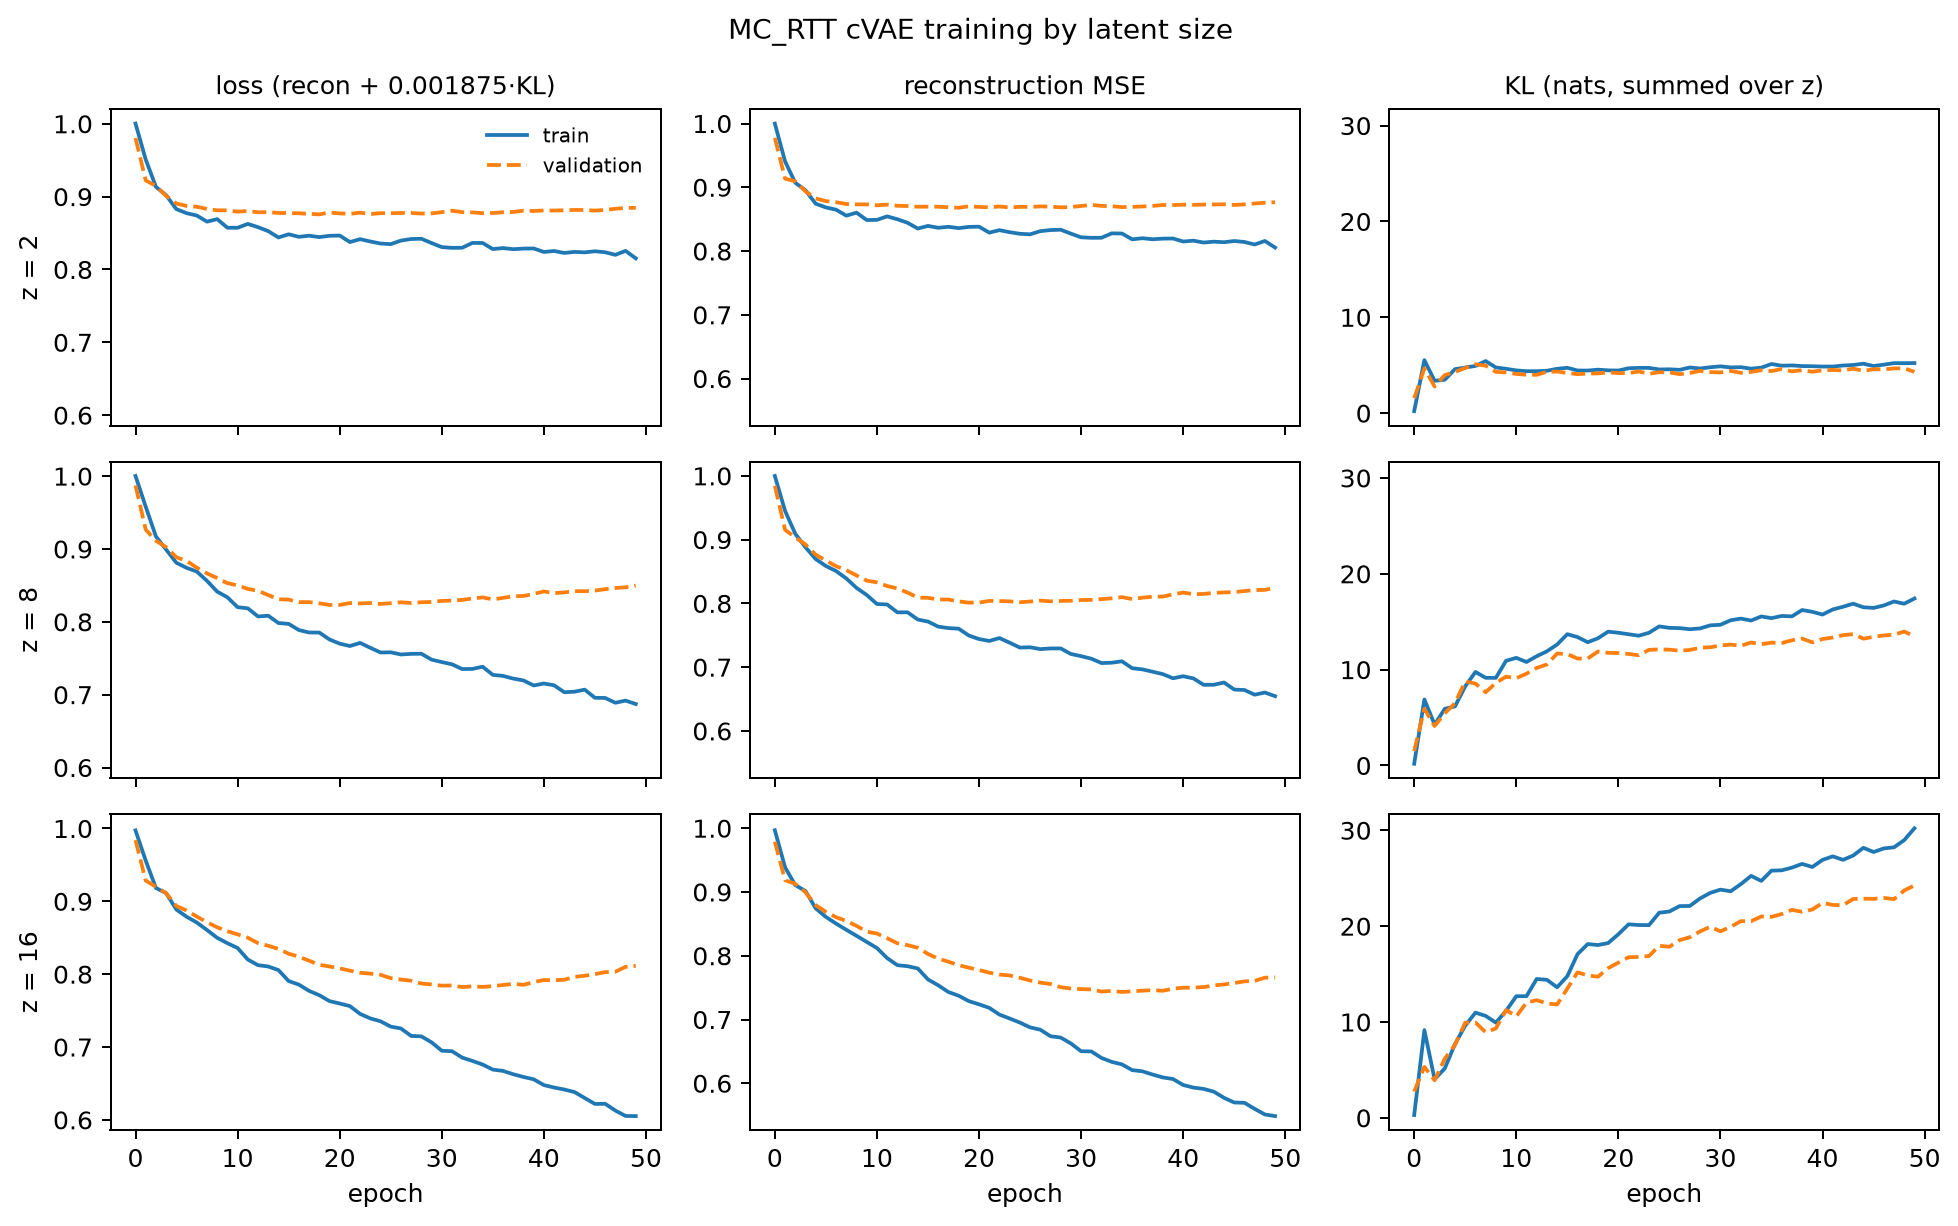
\includegraphics[width=.98\linewidth]{mc_rtt_training.png}
  \caption{Training (solid) and held-out validation (dashed) loss components for each MC\_RTT latent size. Larger models continue to reduce training reconstruction error, while validation reconstruction plateaus or rises modestly late in training.}
  \label{fig:mc-rtt-training}
\end{figure}
\begin{figure}[!htbp]
  \centering
  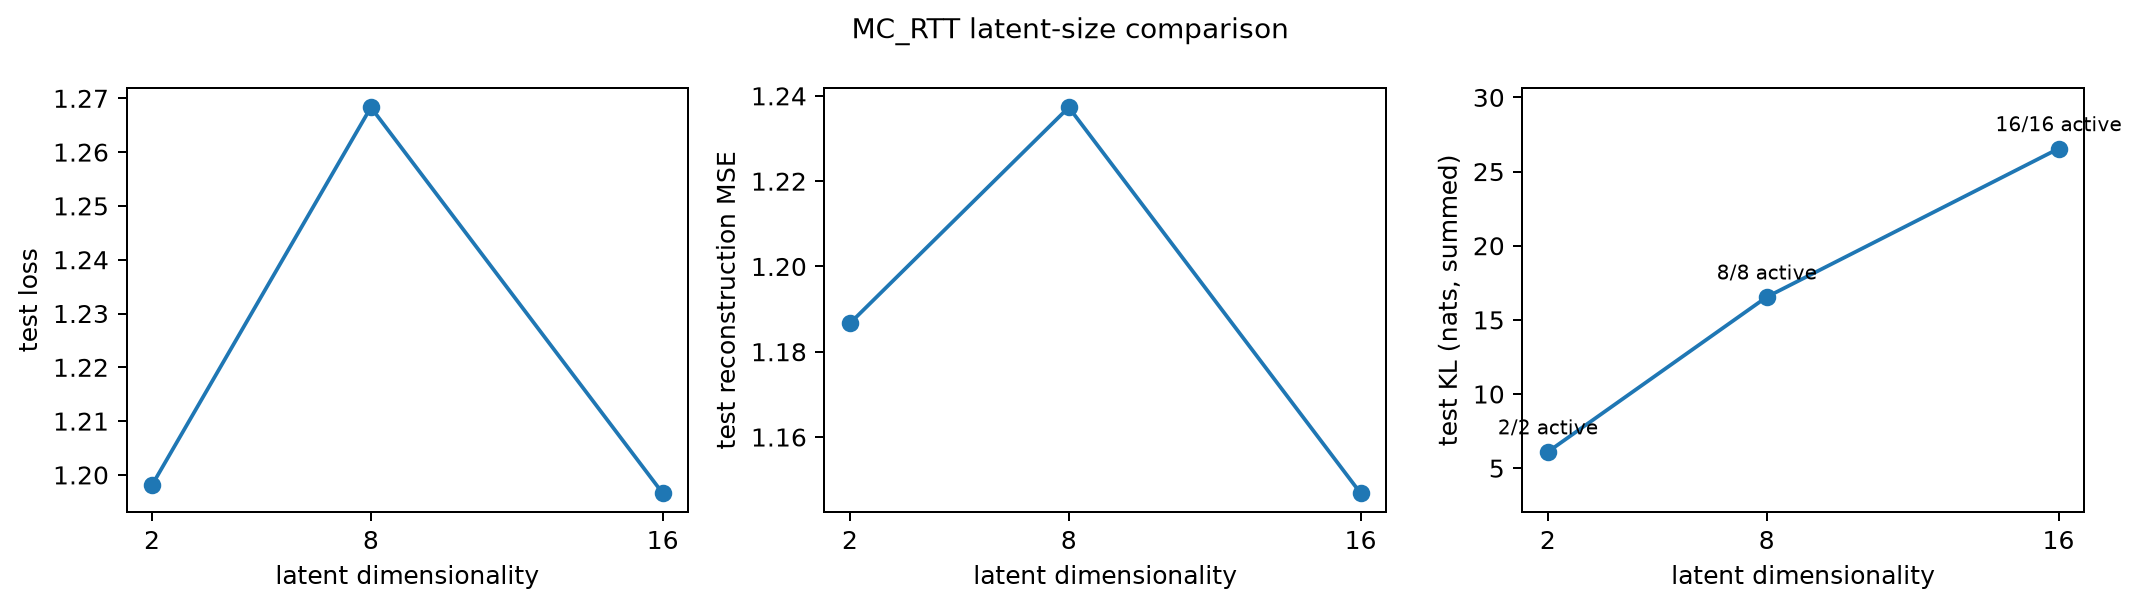
\includegraphics[width=.98\linewidth]{mc_rtt_latent_sweep.png}
  \caption{Final held-out loss, reconstruction error, and KL divergence by latent dimension. All dimensions exceeded the active-dimension threshold, so the larger models did not show posterior collapse under this criterion.}
  \label{fig:mc-rtt-latent-sweep}
\end{figure}
\FloatBarrier

\subsection{Reconstruction and conditional generation}

The observed-versus-reconstructed heatmaps (Figure~\ref{fig:mc-rtt-reconstruction}) show that the cVAE retains broad differences across units and the overall temporal rate pattern, but it replaces sharp trial-specific peaks and troughs with smoother activity.
That smoothing is expected from an MSE decoder trained on smoothed firing-rate features: it is rewarded for predicting a conditional average.

The generated mean rate profiles preserve the broad decline after peak speed in all eight direction conditions (Figure~\ref{fig:mc-rtt-profiles}).
However, the generated amplitude is systematically too low for several directions, especially 0, 1, 5, and 6, and too high for directions 2 and 3.
Therefore, direction conditioning controls coarse population-rate dynamics, but it does not yet reproduce the full direction-specific amplitude pattern.


\begin{figure}[!htbp]
  \centering
  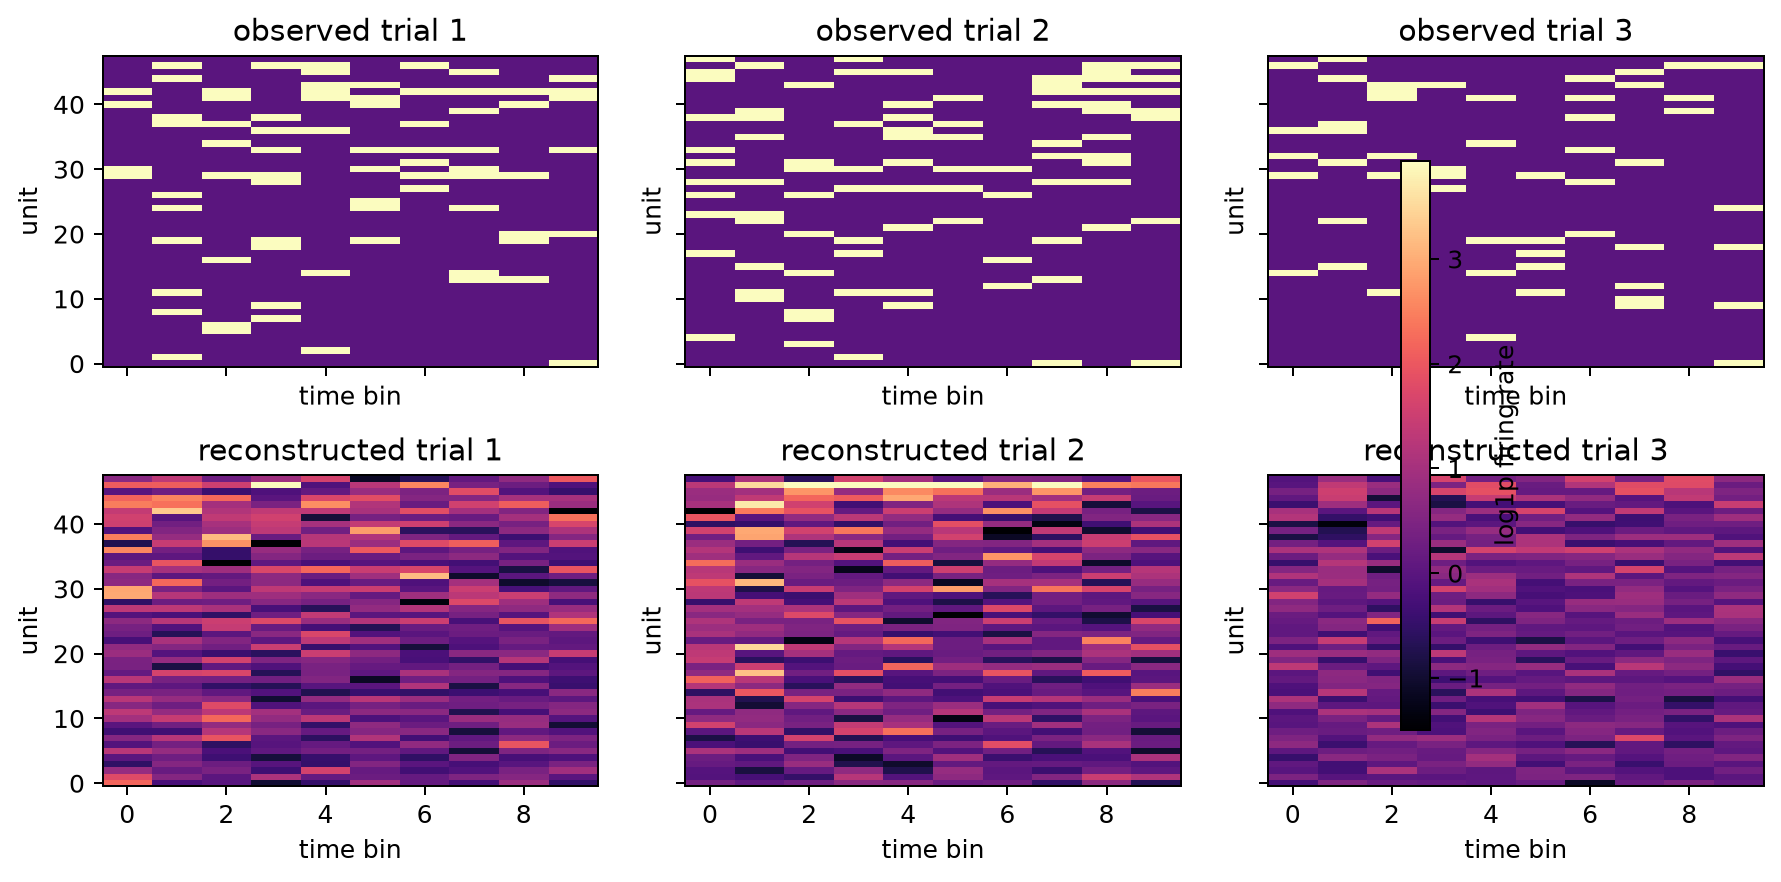
\includegraphics[width=.98\linewidth]{mc_rtt_observed_and_reconstructions.png}
  \caption{Three held-out rate windows (top) and their reconstructions from the $z=8$ cVAE (bottom), displayed on one color scale. The reconstructions retain broad unit- and time-dependent structure but smooth trial-specific variation.}
  \label{fig:mc-rtt-reconstruction}
\end{figure}
\begin{figure}[!htbp]
  \centering
  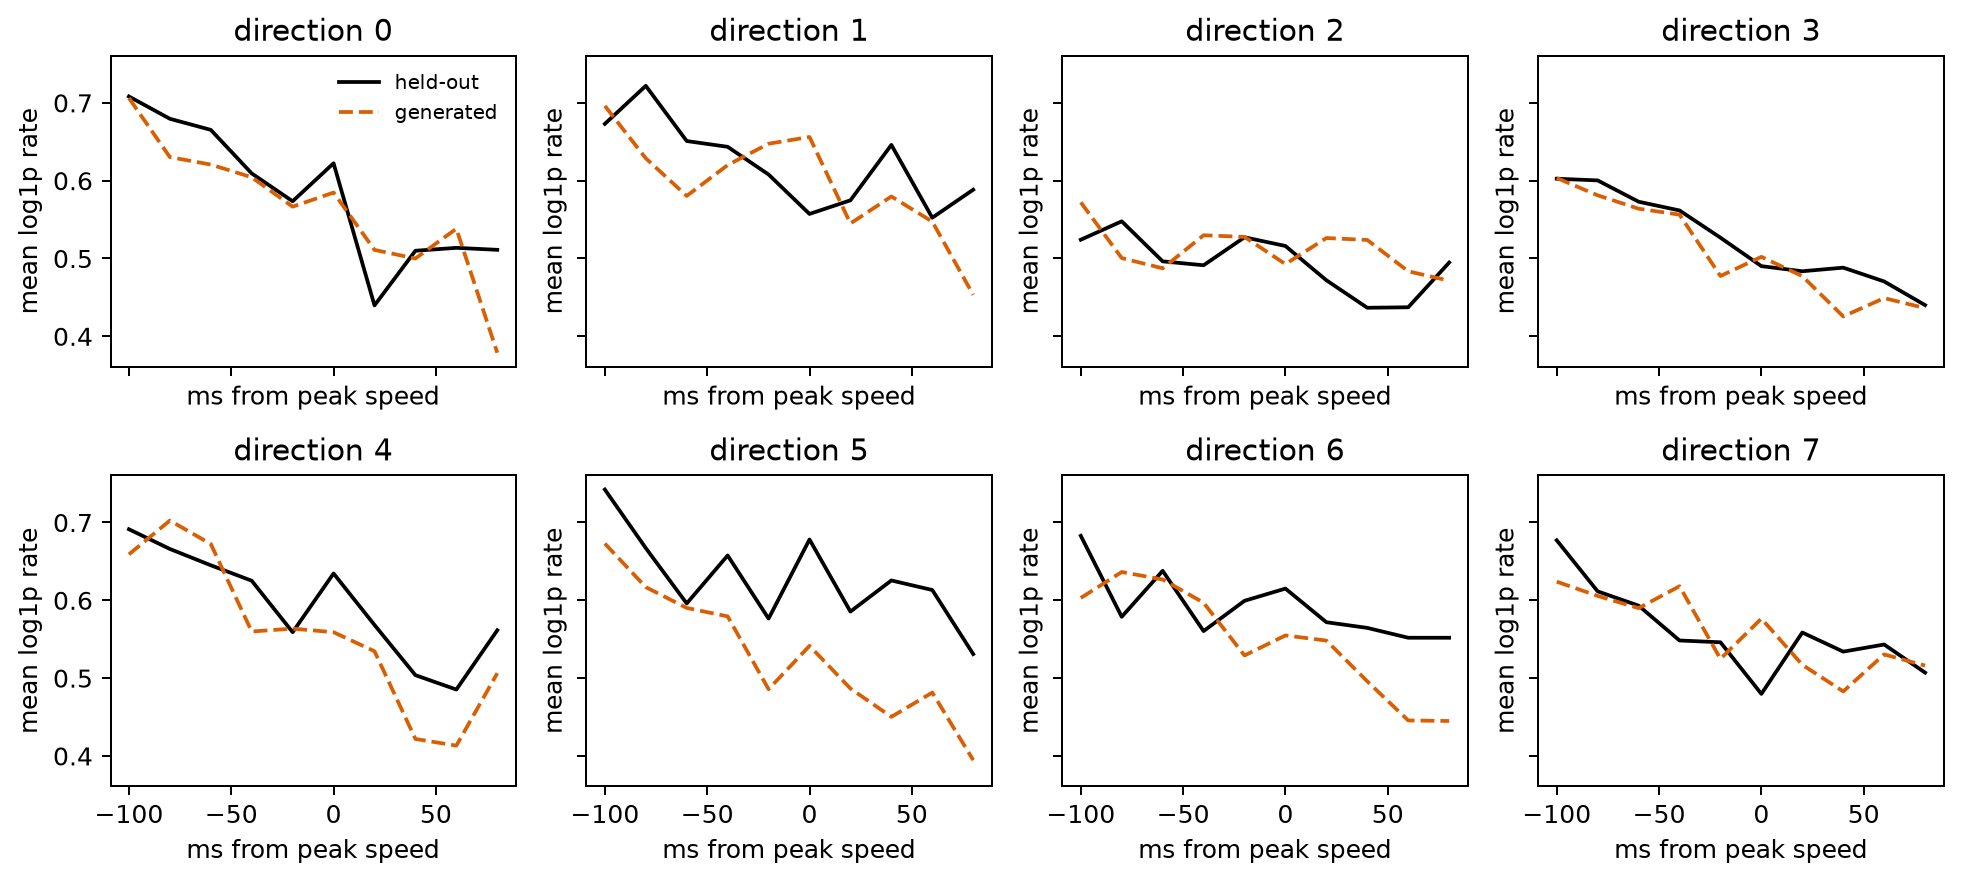
\includegraphics[width=.98\linewidth]{mc_rtt_direction_profiles.png}
  \caption{Mean held-out (black) and generated (dashed orange) log1p firing-rate profiles for each of the eight velocity-direction conditions, using $z=8$.}
  \label{fig:mc-rtt-profiles}
\end{figure}

In the PCA plot (Figure~\ref{fig:mc-rtt-pca}), generated samples occupy the central region of the held-out population cloud but omit many of its most extreme points.
The 16-dimensional samples recover more spread than the smaller models, but all models remain less variable than the held-out data.
The PCA axes are only a visualization of high-dimensional variance; we do not interpret either axis, or any individual latent dimension, as a named neural variable.


\begin{figure}[!htbp]
  \centering
  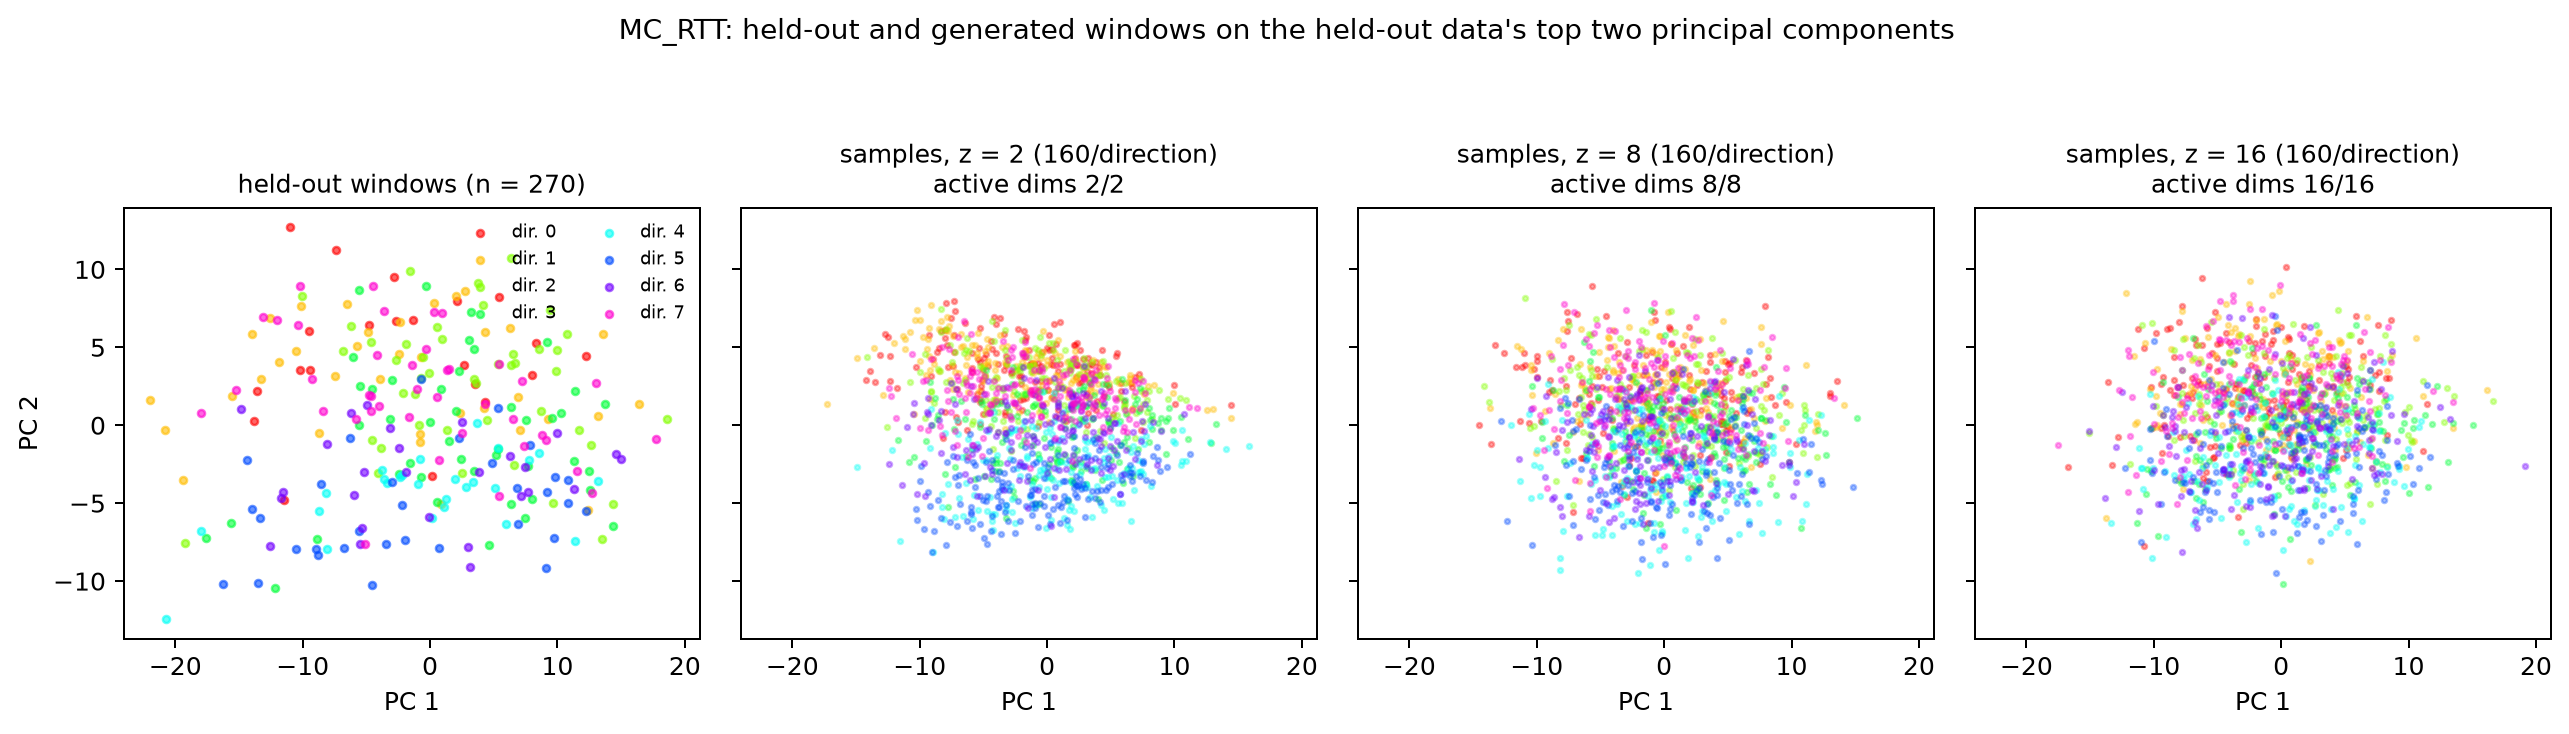
\includegraphics[width=.98\linewidth]{mc_rtt_pca_by_latent.png}
  \caption{Held-out windows and conditional samples projected onto the top two principal components fit to held-out data. Samples cover the central population cloud but underrepresent the most extreme held-out variation.}
  \label{fig:mc-rtt-pca}
\end{figure}

The direction-2 sample comparison (Figure~\ref{fig:mc-rtt-samples-latent}) makes the same point at the unit-by-time level: the generated averages preserve coarse structure, while individual samples remain smoother and less heterogeneous than individual held-out trials.
Overall, the 16-dimensional model had the best final held-out reconstruction metric, while the 8-dimensional model is used as the middle-capacity example for the all-direction visualizations.


\begin{figure}[!htbp]
  \centering
  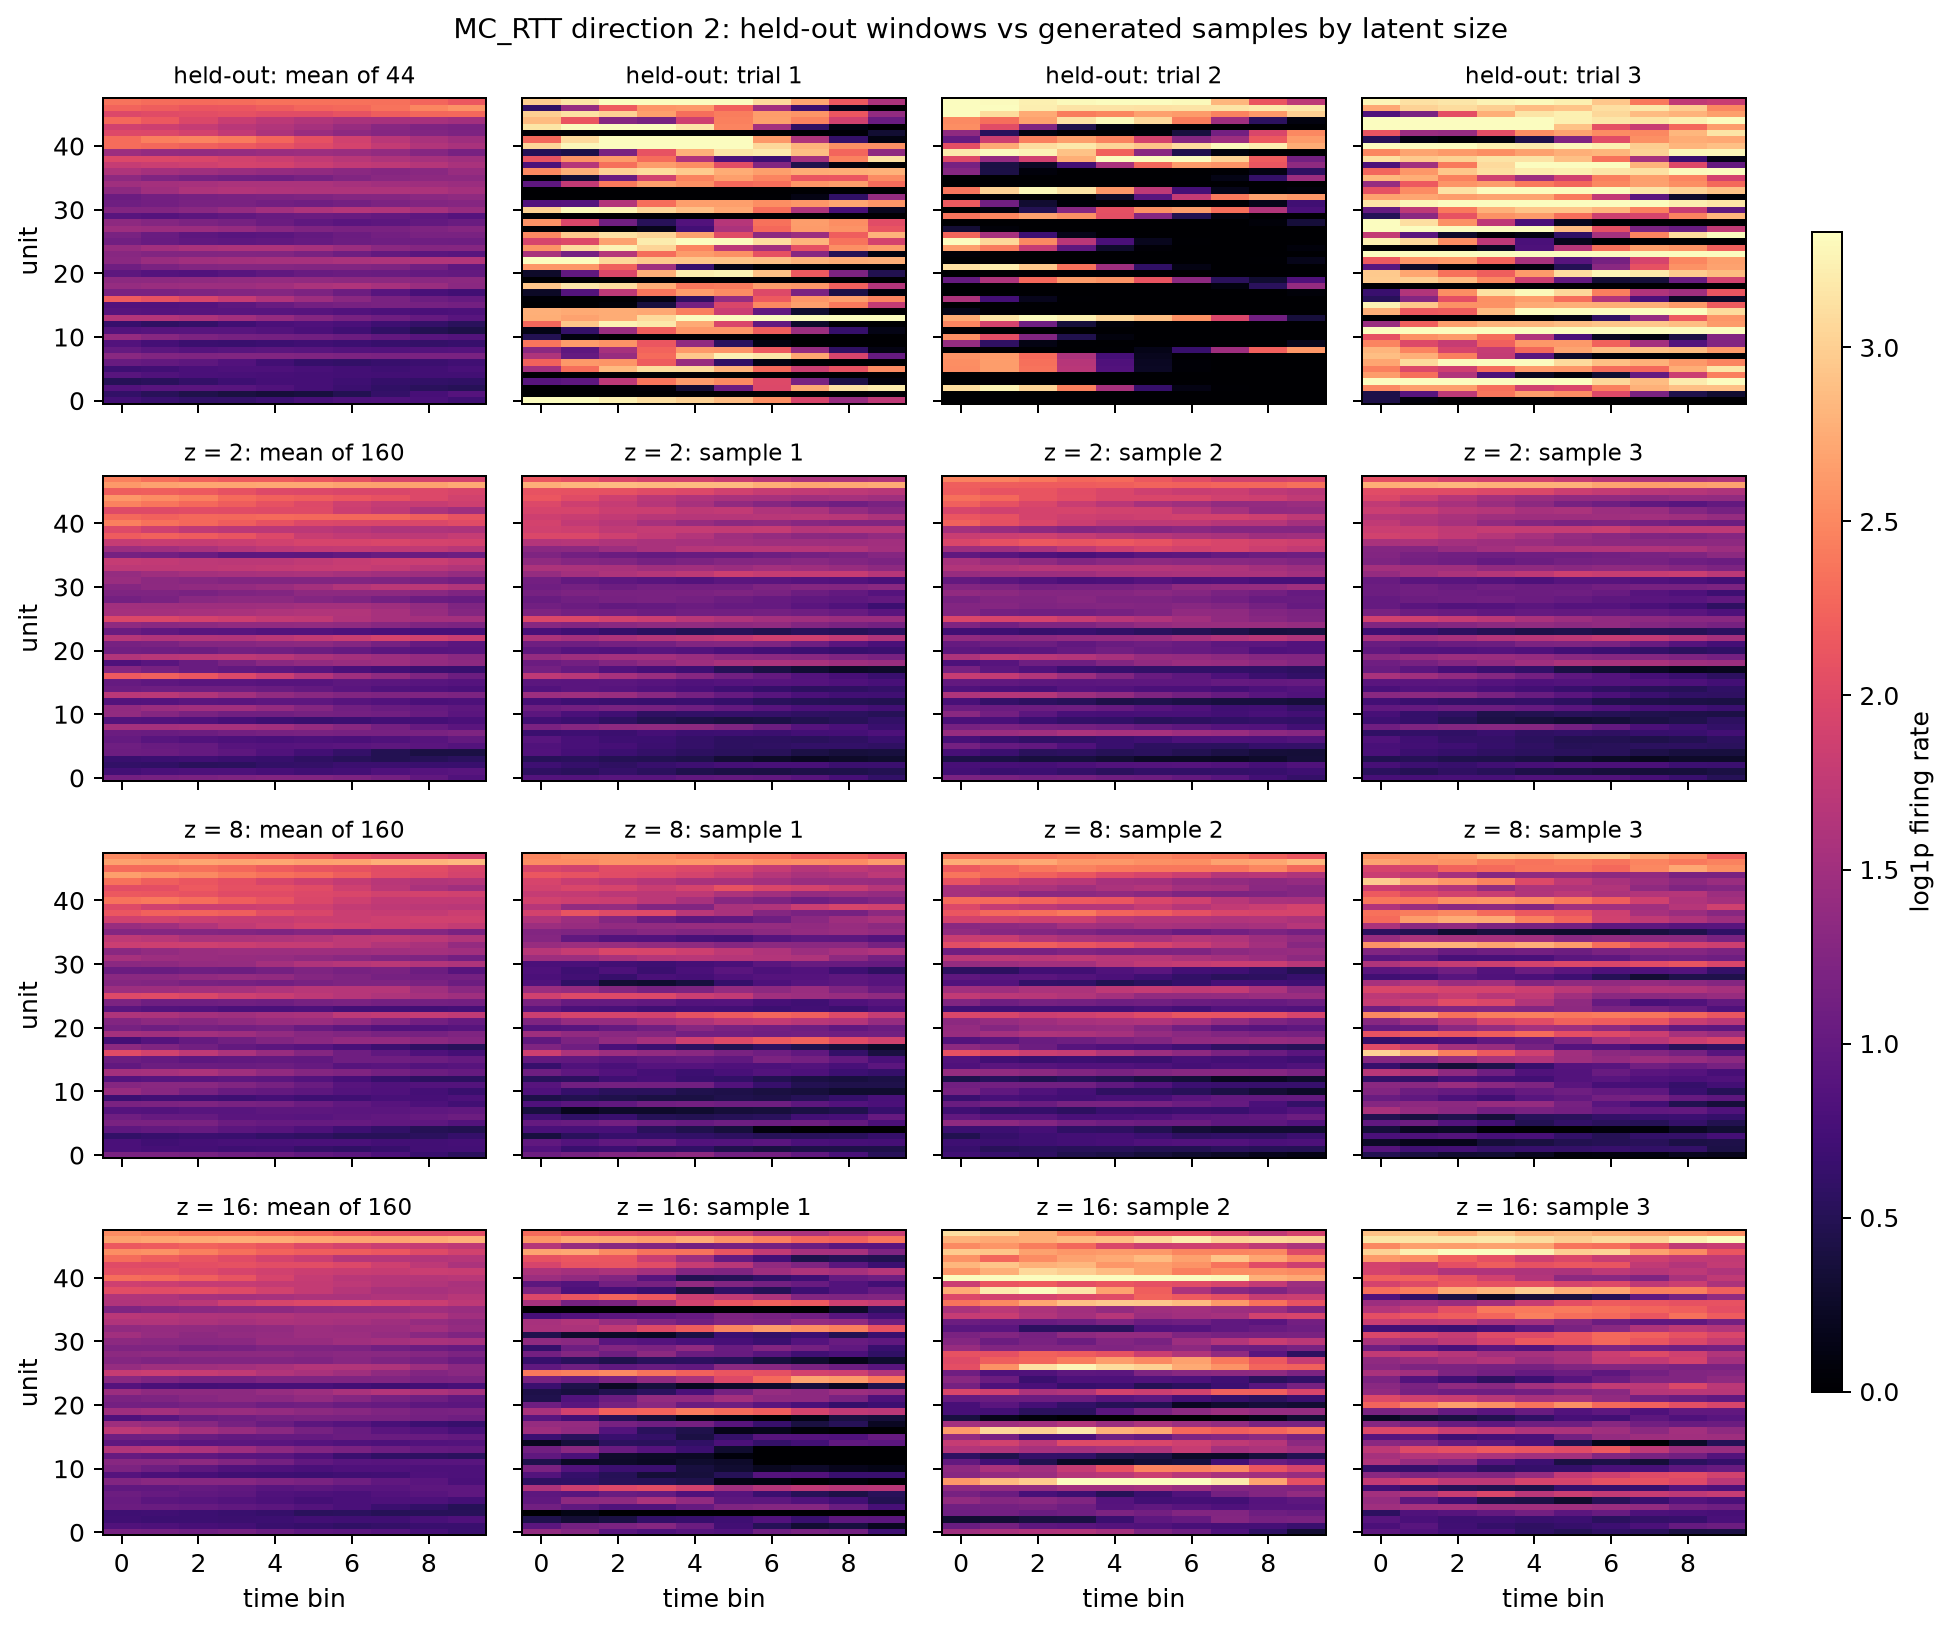
\includegraphics[width=.98\linewidth]{mc_rtt_samples_by_latent.png}
  \caption{Held-out direction-2 windows compared with conditional samples at each latent size. Averaged samples recover broad rate structure; individual samples are smoother and less heterogeneous than held-out trials.}
  \label{fig:mc-rtt-samples-latent}
\end{figure}
\FloatBarrier

\section{Limitations and conclusion}
The main conclusion is narrow: this cVAE learned coarse, direction-conditioned structure in smoothed M1 population-rate windows, but it was not able to reproduce the full variability of the held-out data.
Thus, we conclude that a low reconstruction error alone is not sufficient evidence that a neural generator is realistic.
We also note the PCA and heatmap comparisons show that generated samples are underdispersed and smoother than held-out trials (Figures~\ref{fig:mc-rtt-pca} and \ref{fig:mc-rtt-samples-latent}).
This is *write implications of this here*. 

First, the analysis is not a full model of reaching: it uses one 200-ms window centered on peak speed from each source-provided chunk, so it discards the rest of the reach and does not model transitions across time. 
Because the chunks are not aligned to reaches, a window can also contain only part of a movement.
Second, the inputs are Gaussian-smoothed, log-transformed firing rates rather than raw spike counts or spike times. 
This makes optimization stable, but it necessarily suppresses fine temporal structure before the VAE sees the data.
Third, movement was represented by an eight-level direction label. 
Continuous velocity, target position, and other task variables could explain variation that the latent distribution currently must absorb.
Finally, this result comes from 48 selected held-in units in one recording session and one source-provided train/validation split. 
The training and validation chunks are interleaved, and Gaussian smoothing uses spikes outside each window, so the validation metric may be somewhat optimistic.
It does not establish generalization across sessions, animals, unit selections, seeds, or hyperparameter settings.

The late validation rise for the larger models also suggests that future fits should select checkpoints by validation performance rather than automatically using the final epoch.
A stronger model would generate full reach-aligned sequences with a temporal VAE or state-space model, conditioned on continuous kinematics or target displacement, and use a count-aware likelihood such as Poisson or negative binomial rather than an MSE Gaussian decoder. 
These are possible future directions, but we will not implement these in this assignment. 
Additionally, a stronger evaluation would compare generated and held-out population covariance, pairwise correlations, firing-rate distributions, and kinematic-decoding accuracy for generated samples.
Overall, the latent-dimension sweep shows that added capacity improves held-out reconstruction and remains active (Figure~\ref{fig:mc-rtt-latent-sweep}), but visual sample evaluation showed that capacity alone does not solve the full variability of held-out activity. 


\bibliographystyle{plainnat}
\bibliography{references}
\end{document}
